\begin{SCn}
    \ActivateBG

    \scnheader{Концепция многокомпонентной системы автоматизации исследований}
    \scnidtf{технология сборки систем из компонентов}

    \scntext{примечание}{Технология сборки систем из компонентов является одним из  подходов объектно-ориентированного программирования. Центральным понятием данной технологии является компонент – независимый модуль, который может быть реализован в виде исполняемого файла или динамической библиотеки.}

    \scnheader{Компонент}
    \scnidtf{независимый модуль}
    \scntext{примечание}{В данной работе под компонентом системы автоматизации исследований понимается компонент, который, кроме основной функциональности, обеспечивает реализацию механизма внутренней памяти и предложенного авторами унифицированного интерфейса компонента.Каждый компонент реализует как минимум один интерфейс, который определяет границу взаимодействия компонента с другими компонентами или программами.}

    \scnheader{Интерфейс}
    \scntext{пояснение}{Интерфейс строго специфицирует поведение компонента, благодаря чему компонент может использоваться на основании описания интерфейса при сокрытии (инкапсуляции) от конечного пользователя подробностей реализации компонента}

    \scnheader{Архитекрура многокомпонентной системы автоматизации исследований}
    \begin{scnhaselementset}
        \scnitem{библиотека компонентов, содержащая компоненты с унифицированными интерфейсами}
        \scnitem{управляющий модуль с механизмом интеграции компонентов в единую систему}
    \end{scnhaselementset}
    \scntext{примечание}{Использование унифицированного интерфейса позволяет перестраивать архитектуру системы исследования динамически, без внесения в код компонентов информации о межкомпонентных связях}
    \scntext{схема}{
        \begin{center}
            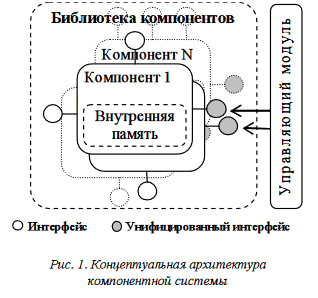
\includegraphics[]{Screenshot 2023-03-20 195659.png}
        \end{center}
    }
    
    \scnheader{Компонент продукционной экспертной системы}
    \scntext{примечание}{Использование продукционной экспертной системы является одним из способов обеспечения пользователя компьютерной поддержкой при принятии решений на основе знаний эксперта. Как компонент продукционная экспертная система может использоваться либо для решения задач предметной области (связанных с логическим выводом), либо для интеллектуализации работы программной системы (возможность программной системы осуществлять самонастройку с использованием внутренних баз знаний). Решение подобных задач требует предметных (модель предметной области) и проблемных (принципиальные методы решения проблемы на основе модели предметной области) знаний. Предметные знания зависят от предметной области, проблемные остаются неизменными при выборе любой предметной области. На этом принципе организована реализация оболочек экспертных систем. Предлагается создать архитектуру компонента продукционной системы, обеспечивающую решение широкого круга задач на основе использования множества баз знаний. Предполагается, что базы знаний могут быть накоплены различными пользователями и описаны на независимом от машины вывода языке. В настоящее время существуют как коммерческие, так и свободно распространяемые оболочки продукционных экспертных систем (CLIPS [5], JESS, OPS5), с помощью которых можно реализовать механизм рассуждения на основе продукций. В связи с этим наиболее рациональным представляется реализация данного компонента на основе уже существующей машины вывода. В данной работе для этой цели выбрана свободно распространяемая система CLIPS (C Language Integrated Production System).}

    \scnheader{Управляющий модуль}
    \scntext{примечание}{Для применения CLIPS в качестве компонента системы автоматизации исследований необходимо создать модуль управления данной системой. Модуль управления с помощью механизма компонентной обертки обеспечивает реализацию унифицированного интерфейса компонента и механизма внутренней памяти для управляемой программной системы.}

    \scnheader{Функции модуля управления}
    \begin{scnrelfromset}{разбиение}
    \scnitem{не зависимые от специфики компонента}
    \begin{scnhaselementset}
        \scnitem{предоставление информации о свойствах управляемой системы и реализуемых ею функциях;}
        \scnitem{прямое и обратное преобразование полученной извне информации в формат, используемый управляемой системой;}
        \scnitem{управление состоянием параметров управляемой (контролируемой) системы}
    \end{scnhaselementset}
    
    \scnitem{зависимые}
    \begin{scnhaselementset}
        \scnitem{создание базы знаний в виде набора правил и классов фактов в обобщенном виде;}
        \scnitem{преобразование правил и фактов из обобщенного вида к формату машины вывода CLIPS;}
        \scnitem{управление процессом вывода
            \begin{scnhaselementset}
                \scnitem{формирование рабочей базы знаний на основе обобщенного представления (вида)}
                \scnitem{передача рабочей базы знаний в машину вывода (загрузка ее в рабочую память);}
                \scnitem{получение результатов и преобразование их в обобщенный вид.}
        \end{scnhaselementset}}
    \end{scnhaselementset}
\end{scnrelfromset}

\scntext{примечание}{Необходимо отметить, что при реализации компонента продукционной экспертной системы предлагается использовать двухуровневую модель представления правил и фактов: первый уровень – логический: представление фактов и правил в виде, не зависимом от конкретной машины вывода (обобщенный вид); второй уровень – физический: представление фактов и правил в формате опреде- ленной машины вывода, например CLIPS. Использование подобной двухуровневой модели позволяет значительно снизить затраты на разработку нового компонента при выборе другой машины вывода.}

\scnheader{Компонент продукционной экспертной системы}
\begin{scnhaselementset}
     \scnitem{
        Модуль преобразования\par
        \scntext{примечание}{обеспечивает не только приведение правил и фактов из обобщенного вида к языку конкретной машины вывода, например, к формату CLIPS, но и обратное преобразование. Сформированная в результате преобразования рабочая база знаний подключается к машине вывода путем загрузки рабочей базы знаний в рабочую память. Реализация данного модуля зависит от специфики используемой машины вывода и нуждается в изменении в случае замены машины вывода при создании нового компонента.}}
     \scnitem{
        Продукционная машина вывода\par
        \scntext{примечание}{осуществляет процесс рассуждения (логического вывода) по правилам. При реализации данного модуля будет использоваться динамическая библиотека, реализующая машину вывода CLIPS.}}
\end{scnhaselementset}
\scntext{примечание}{предназначен для работы (выполнение операций создания, модификации и удаления) с фактами и правилами, представлен-ными в обобщенном виде. При этом правила и факты могут быть как абстрактными (образцы правил и фактов), так и конкретными (экземпляры правил и фактов). Факты и правила группируются согласно их предметной классификации, образуя базы знаний и формируя таким образом сферы своего применения. Каждая база знаний имеет уникальное имя и рассматривается компонентом в качестве предоставляемой им функции, доступ к которой осуществляется через унифицированный интерфейс компонента.}
\scntext{схема}{
    \begin{center}
        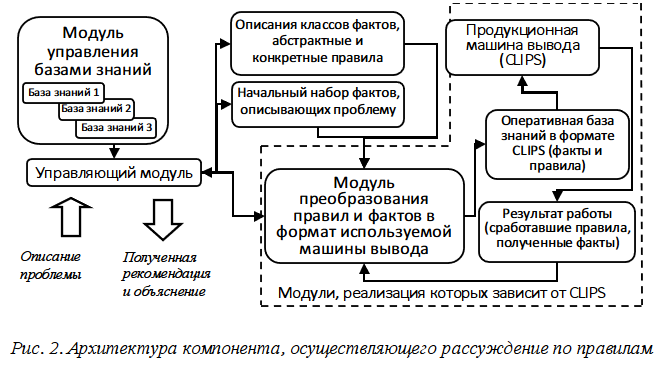
\includegraphics[]{Screenshot 2023-03-21 094429.png}
    \end{center}
}

\scnheader{Продукционное правило}
\scntext{теоретико-множественная модель}{Q; P; A→B; N.\\
    \scntext{примечание}{Для представления продукционного правила в обобщенном виде используется следующая теоретико-множественная модель: (i): Q; P; A→B; N, где i – имя продукции; Q – сфера применения продукции; P – предусловие (условие применимости ядра продукции); A→B – ядро продукции (Если ... То ...); N – постусловие продукции.}
}
    \begin{center}
        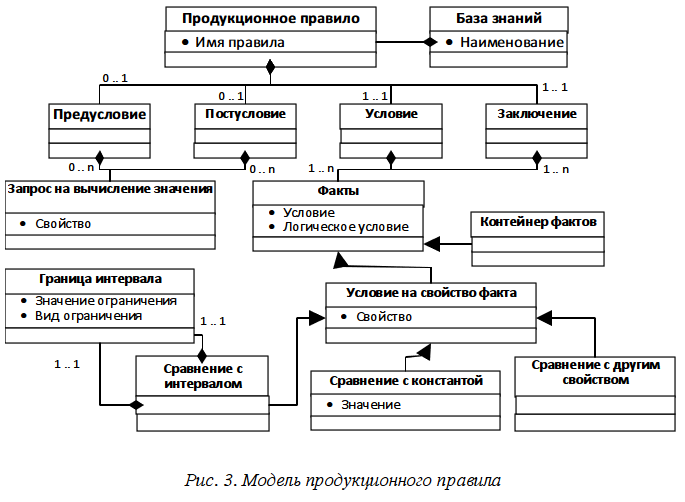
\includegraphics[]{Screenshot 2023-03-21 094514.png}
    \end{center}
}

\newpage
\end{SCn}